\documentclass[a4paper,11pt,headinclude=true,headsepline,parskip=half,DIV=13]{scrartcl}

% font, style, etc.
\usepackage[utf8]{inputenc} % defines
\usepackage[automark]{scrlayer-scrpage}
\usepackage{csquotes}
\usepackage{xspace} % proper space after macros with 0 args

% mathematics
\usepackage{amsmath}
\usepackage{amssymb}

% figures, tables, etc.
\usepackage{hyperref} %
\usepackage{graphicx}
\usepackage{tikz}
\usepackage{pgf}
\usepackage{xcolor}
\usepackage{placeins} % -> floatbarrier
\usepackage{siunitx}  % -> handling of units
%\usepackage[printwatermark]{xwatermark}
%\newwatermark[allpages,color=red!50,angle=45,scale=1.8,xpos=0,ypos=0]{\textsf{DRAFT ONLY,NOT APPROVED}}

% code
\usepackage{listings}
\lstset{
language=Python, 
backgroundcolor = \color{light-gray},
basicstyle=\scriptsize\sffamily,
stringstyle=\color{orange},
breaklines=true,
numberstyle=\tiny\color{gray},
keywordstyle=\bfseries\color{dark-blue}\textit, % print keywords dark-blue
commentstyle=\color{dark-green}, % print comments dark-green
showstringspaces=false} % spacing between strings not showed

\newcommand{\listcode}[3]{\lstinputlisting[numbers=left,firstnumber=#1,firstline=#1,lastline=#2]{#3}}
\newcommand{\listcodeplot}[2]{\listcode{#1}{#2}{../sim/01_car_example_plotting.py}}
\newcommand{\listcodeanim}[2]{\listcode{#1}{#2}{../sim/02_car_example_animation.py}}

% others
\usepackage{acronym}

% theorems
\newtheorem{defi}{Definition}[section]

% setup the appearance of links
\hypersetup{
    colorlinks = true, % false -> red box arround links (not very nice)
    linkcolor={blue!100!black},
    citecolor={blue!100!black},
    urlcolor={blue!100!black},
}

% manage glossaries
% Call makeglossaries on a command prompt after LaTeX compiling,
% the re-run LaTeX
\usepackage{glossaries}
\setacronymstyle{long-short}
\makeglossaries
\newacronym{ivp}{IVP}{initial value problem}
\newacronym{ode}{ODE}{ordinary differential equation}

% define shortcuts
\newcommand{\ad}{\mathrm{ad}}
\renewcommand{\d}{\mathrm{d}} % d vor differential forms
\newcommand{\NV}{{\cal N}\,}
\newcommand{\rang}{\mathrm{rang}}
\newcommand{\im}{\mathrm{im}}
\newcommand{\spann}{\mathrm{span}}
\newcommand{\R}{\mathbb{R}} %  set of real numbers
\newcommand{\py}{\emph{Python}\xspace}
\newcommand{\scipy}{\emph{SciPy}\xspace}
\newcommand{\numpy}{\emph{NumPy}\xspace}
\newcommand{\mpl}{\emph{Matplotlib}\xspace}
\newcommand{\uu}{\mathbf{u}}
\newcommand{\f}{\mathbf{f}}
\newcommand{\x}{\mathbf{x}}
\newcommand{\y}{\mathbf{y}}
\newcommand{\z}{\mathbf{z}}
\newcommand{\xZero}{\mathbf{x}_0}

% color definitions
\definecolor{light-gray}{gray}{0.95}
\definecolor{dark-blue}{rgb}{0, 0, 0.5}
\definecolor{dark-red}{rgb}{0.5, 0, 0}
\definecolor{dark-green}{rgb}{0, 0.5, 0}
\definecolor{gray}{rgb}{0.5, 0.5, 0.5}

% Avoid ugly indentations in footnotes.
\deffootnote[1em]{1em}{0em}{%
\textsuperscript{\thefootnotemark}%
}

% ----------------------------------------------------------------------------
\subject{\py for simulation, animation and control}
\title{Model of a Kinematic Vehicle}
\subtitle{An introductory tutorial for simulation of dynamic systems}
\author{Max Pritzkoleit\thanks{Institute for Control Theory, Faculty of Electrical and Computer Engineering, Technische Universität Dresden, Germany} \and Jan Winkler\footnotemark[1]}
\publishers{}
\date{\today}
% ----------------------------------------------------------------------------

% Headings
\pagestyle{scrheadings}
\ihead{\leftmark}
\chead{}
\ohead{Page \pagemark}
\ifoot{}
\cfoot{Python Control Tutorial 1}
\ofoot{}

\begin{document}

\maketitle




\tableofcontents

\newpage

\section{Introduction}
The goal of this tutorial is to teach the usage of the programming language \py as a tool for developing and simulating control systems  represented by nonlinear \glspl{ode}. The following topics are covered:
\begin{itemize}
\item Implementation of the model in \py,
\item Simulation of the model,
\item Presentation of the results.
\end{itemize}
\textbf{\py source code file: \texttt{01\_car\_example\_plotting.py}}

Later the simulation is extended by a visualization of the moving vehicle and some advanced methods for numerical integration of \glspl{ode}.

If not familiar with the handling of containers and arrays in \py one should refer to the \href{http://cs231n.github.io/python-numpy-tutorial/#python-containers}{\py List-Dictionary-Tuple tutorial} and the \href{http://cs231n.github.io/python-numpy-tutorial/#numpy}{NumPy Array tutorial}. If the reader is completely new to \py the very basic introduction on \href{https://www.tutorialspoint.com/python/index.htm}{tutorialspoint} maybe helpful as a first starting point.

\section{Kinematic model of a vehicle}
\label{sec:model}
\begin{figure}[ht]
  \centering
  \def\svgwidth{0.7\textwidth}
  \input{img/car-like_mobile_robot.pdf_tex}
  \caption{Car-like mobile robot}
  \label{fig:car}
\end{figure}
Given is a nonlinear kinematic model of a car-like mobile robot, cf.~Figure \ref{fig:car}, with the following system variables: position $(y_1, y_2)$ and orientation $\theta$ in the plane, the steering angle $\phi$ and the vehicle's lateral velocity $v=\left| \mathbf{v} \right| $: 
\begin{subequations}\label{eq:syseq}
\begin{alignat}{2}
\dot{y}_1(t)&=v \cos (\theta(t)) &\qquad y_1(0) &= y_{10}\\
\dot{y}_2(t)&=v \sin (\theta(t)) &\qquad y_2(0) &= y_{20}\\
\dot{\theta}(t) &= \frac{1}{l}v(t)\tan(\phi(t)) &\qquad \theta(0) &= \theta_{0}.
\end{alignat}
\end{subequations}
The initial values are denoted by $y_{10}$, $y_{20}$, and $\theta_0$, respectively, and the length of the vehicle is given by $l$. The velocity $v$ and the steering angle $\phi$ can be considered as an input acting on the system.

To simulate this system \eqref{eq:syseq} of first order \glspl{ode}, one has to introduce a state vector $\x=(x_1,x_2,x_3)^\mathrm{T}$ and a control vector $\uu=(u_1,u_2)^\mathrm{T}$ as follows:
\begin{subequations}
\begin{alignat}{2}
x_1 &:= y_1 &\qquad u_1 &:= v\\
x_2 &:= y_2 &\qquad  u_2 &:= \phi \:. \\
x_3 &:= \theta
\end{alignat}
\end{subequations}
Now, the \gls{ivp} \eqref{eq:syseq} can be expressed in the general form $\dot{\x}(t)=\f(\x(t),\uu(t))$ with $\x(0) = \xZero$:
\label{eq:ss_system}
\begin{align} \label{eq:odesys}
\underbrace{\begin{pmatrix} \dot{x}_1(t) \\ \dot{x}_2(t) \\ \dot{x}_3(t) \end{pmatrix}}_{\dot{\x}(t)} = \underbrace{\begin{pmatrix}  u_1(t) \cos(x_3(t)) \\ u_1(t) \sin(x_3(t)) \\ \frac{1}{l}u_1(t) \tan(u_2(t)) \end{pmatrix}}_{\f(\x(t),\uu(t))} \qquad \x(0) = \xZero.
\end{align}
Usually, this explicit formulation of the \gls{ivp} is the basis for implementing a system simulation by numerical integration. In the following a simulation using \py is setup which shows the dynamic behavior of the vehicle when driving with a continously decreasing velocity under a constant steering angle. Of course, in this simple case, the result is known in advance: The vehicle will drive on a circle until it stops for $v = 0$. In the following the \py-script for simulating the system will be derived step by step.


\section{Libraries and Packages}
Neither the numerical solution of the \gls{ivp} \eqref{eq:syseq} nor the presentation of the results can be done comfortably in pure \py. To overcome this limitation separate packages for array handling, numerical integration, and plotting are provided. Under \py such packages should be imported at the top of the executed script\footnote{It is also possible to import them elsewhere in the code but following the official style guide PEP8 ``imports are always put at the top of the file, just after any comments and docstrings, and before globals and constants''.}.

The most relevant packages for the simulation of control systems are

\begin{itemize}
\item \href{http://www.numpy.org/}{\numpy} for array handling and mathematical functions,
\item \href{https://docs.scipy.org/doc/scipy/reference/}{\scipy} for numerical integration of \glspl{ode} (and a lot of other stuff, of course),
\item \href{https://matplotlib.org/}{\mpl} for plotting.
\end{itemize}

It is good practice to connect the imported packages with a namespace so it can be easily seen in the code which function comes from where. For example, in case of \numpy the following statement imports the package \numpy and ensures that every function from \numpy is addressed by the prefix \texttt{np.}:
\listcodeplot{2}{2}
For frequently used functions like \texttt{cos(...)}, \texttt{sin(...)}, and \texttt{tan(...)} it is annoying to prefix them like \texttt{np.cos(...)} each time. To avoid this one can directly import them as 
\listcodeplot{3}{3}
To solve the \gls{ivp} \eqref{eq:ss_system} the library \scipy with its sub-package \emph{integrate} offers different solvers:
\listcodeplot{4}{4}
For plotting the output of the simulation results the library \mpl with its sub-package \emph{pyplot} introduces a user experience similar to \emph{MATLAB} into \py:
\listcodeplot{5}{5}


\section{Storing parameters}
In simulations usually a lot of parameters describing the system or the simulation setup have to be handled. It is a good idea to store these parameters as attributes in a structure so it is not necessary to deal with several individual variables holding the values of the parameters. Basically, such a structure can be an instance of an empty class derived from \texttt{object} to which members holding the parameter values are subsequently assigned:
\listcodeplot{8}{15}
Similarily this can be done with the simulation parameters:
\listcodeplot{17}{21}

Alternatively, one could use the datatype \emph{dictionary}. However, the resulting keyword notation (e.g., \texttt{para["l"]} instead of \texttt{para.l}) in the code using the parameters is quite annoying.


\section{Simulation with \scipy's integrate package} \label{sec:simulation}

\subsection{Implementation of the model} \label{sec:implementation-model}
In order to simulate the \gls{ivp} \eqref{eq:odesys} using the numerical integrators offered by \scipy's integrate package a function returning the right hand side of \eqref{eq:odesys} evaluated for given values of $\x$, $\uu$ and the parameters has to implemented:
\listcodeplot{24}{44}
The \texttt{ode} functions calls the control law function \texttt{control} calculating values for $v$ and $\phi$ depending on the state $\x$ and the time $t$. As a first heuristic approach, the vehicle is driven with a constant steering angle while continously reducing the speed from \SI{0.5}{\meter\per\second} to zero. Later, an arbitrary function, for expample a feedback law $\uu=k(\x)$, can be implemented.
\listcodeplot{47}{60}
It is important that the function needs to handle also time arrays as input in order to calculate the control for a bunch of values at once (not during the numerical integration but later for analysis purposes). That's why \numpy's array capable \href{https://docs.scipy.org/doc/numpy/reference/generated/numpy.maximum.html}{maximum function} is used here with appropriately adjusted shape of \texttt{u2}.

Furthermore, attention has to be paid how the two functions above are documented. The text within the \texttt{"""} is called \emph{docstring}. Tools like \href{http://www.sphinx-doc.org/en/stable/}{Sphinx} are able to convert these into well formatted documentations. Docstrings can be written in several ways. Here the so-called \href{https://sphinxcontrib-napoleon.readthedocs.io/en/latest/example_google.html}{Google Style} is used.


\subsection{Solution of the initial value problem using \scipy}
Having implemented the system dynamics the numerical integration of system \eqref{eq:odesys} can be performed. At first, a vector \texttt{tt} specifying the time values at which one would like to obtain the computed values of $\x$ has to be defined. Then the initial vector $\xZero$ is defined and the  \href{https://docs.scipy.org/doc/scipy/reference/generated/scipy.integrate.odeint.html}{odeint} function of the \scipy \emph{integrate} package is called to perform the simulation\footnote{Consider using the more advanced integrators offered by \scipy, see Section \ref{sec:ScipyLambda}.}. The function \texttt{odeint} implements an adaptive variable step solver although it outputs the result at equally spaced time steps defined by the user in \texttt{tt} here. The output is an array of shape \texttt{len(tt)}$\times$\texttt{len(x0)}. Finally, the control input values are calculated from the obtained trajectory of $\x$ (the values for $\uu$ in the \texttt{ode} function cannot be directly saved because the function is also repeatedly called between the specified time steps by the solver).
\listcodeplot{135}{143}
Note that the interval specified by \texttt{np.arange} is open on the right hand side. Hence, \texttt{dt} is added to obtain also values for $\x$ at \texttt{tf}. 


\section{Plotting using \mpl} \label{sec:plot}
Usually one wants to publish the results with descriptive illustrations. For this purpose the required plotting instructions are encapsulated in a function. This way, one can easily modify parameters of the plot, for example figure width, or if the figure should be saved on the hard drive.
\listcodeplot{63}{132}
Having defined the plotting function, one can execute it passing the calculated trajectories.
\listcodeplot{145}{148}
The result can be found in Figure \ref{fig:state_traj}. Other properties of the plot, like line width or line color and many others, can be easily changed. One may refer to the \href{https://matplotlib.org/api/pyplot_summary.html}{documentation of \mpl} or consult the exhaustive \href{https://matplotlib.org/gallery/index.html}{\mpl example gallery}.
\begin{figure}[h!]
\label{fig:state_traj}
   \centering      
   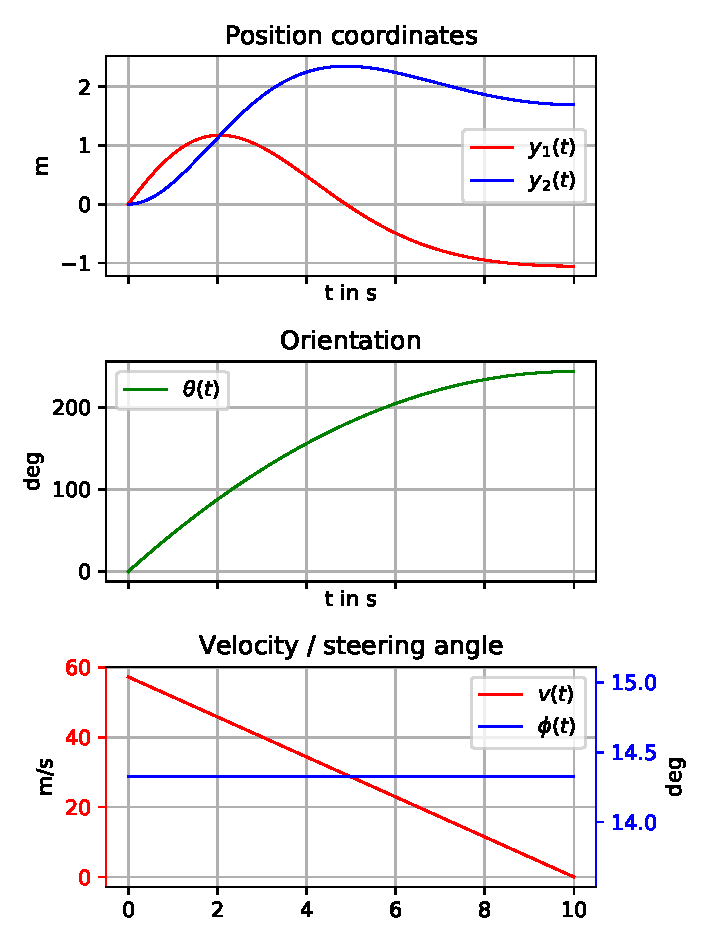
\includegraphics[width=0.8\textwidth]{img/state_trajectory.pdf}      
 \caption{State and control trajectory plot created with \mpl.}
 \label{fig:Test}
\end{figure} 


%\FloatBarrier

\section{Animation using \mpl} \label{sec:animation}

\textbf{\py source code file: \texttt{02\_car\_example\_animation.py}}

Plotting the state trajectory is often sufficient, but sometimes it can be helpful to have a visual representation of the system dynamics in order to get a better understanding of what is actually happening. This applies especially for mechanical systems. \mpl provides the sub-package \texttt{animation}, which can be used for such a purpose. One has to add
\listcodeanim{6}{6}
at the top of the code used in the previous sections. Under Windows it might be necessary to explicitely specify the path to the \emph{FFMPG} library, e.g.:
\begin{lstlisting}
plt.rcParams['animation.ffmpeg_path'] = 'C:\\path\\to\\ffmpg\\ffmpeg.exe'
\end{lstlisting}
\emph{FFMPG} can be downloaded from \url{https://www.ffmpeg.org/download.html}.

All processing steps required for the animation are encapsulated in a function called \texttt{car\_animation()}. At first this functions creates a figure with two empty plots into which the car and the curve of the trajectory dependung on the state $\x$, the control input $\uu$ and the parameters are plotted later:
\listcodeanim{137}{165}
The handles \texttt{h\_x\_traj\_plot} and \texttt{h\_car} are used later to draw onto the axes.

In the animation a representation of the vehicle has to be subsequently drawn. This is done by plotting lines. All lines that represent the vehicle are defined by points, which depend on the current state $\x$ and the control input $\uu$. Hence, one needs a function inside \texttt{car\_animation()} that maps from $\x$ and $\uu$ to a set of points in the $(Y_1,Y_2)$-plane using geometric relations and passes these to the plot instance \texttt{car}:
\listcodeanim{167}{223}
Note that \texttt{car\_plot} is in the scope of the \texttt{car\_animation} function and, hence, has full acess to the handle \texttt{h\_car} here.

Two further functions are required: \texttt{init()} and \texttt{animate(i)}. They will be later called by \mpl to initialize and perform the animation. The \texttt{init()}-function defines which objects change during the animation, in this case the two axes the handles of which are returned:
\listcodeanim{225}{234}

The \emph{animate(i)}-function assigns data to the changing objects, here the car, trajectory plots and the simulation time (as part of the axis):
\listcodeanim{236}{250}

Finally an object of type \texttt{FuncAnimation} is instancciated. It is provided by the animation subpackage of \mpl. It takes  \texttt{animate()} and \texttt{init()} as argumets in the constructor:
\listcodeanim{252}{258}

Note that all lines from 138 to 258 belong to the function \texttt{car\_animation}!

Now the system can be simulated with animated results.
\listcodeanim{274}{277}

\begin{figure}[ht]
  \centering
  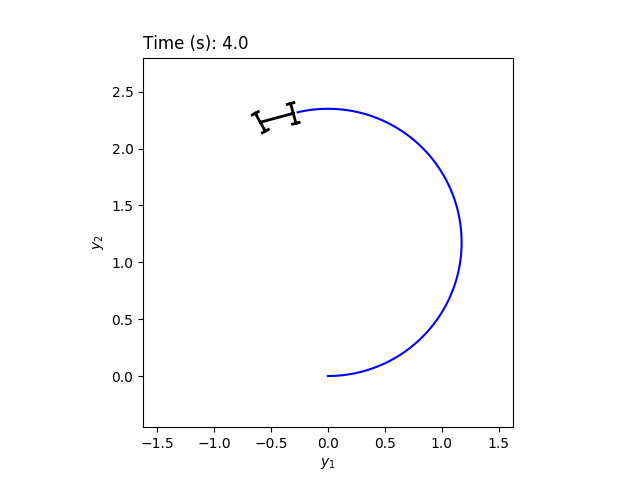
\includegraphics[width=0.7\textwidth]{img/animation}
  \caption{Car animation}
  \label{fig:animation}
\end{figure}
        



\section{Simulation with \scipy's new \emph{solve\_ivp} module and the \emph{lambda} function}\label{sec:ScipyLambda}

\textbf{\py source code file: \texttt{03\_car\_example\_scipy\_solve\_ivp.py}}

In addition to the solution in \autoref{sec:simulation} using \texttt{odeint}, \scipy's integrate package contains some newer and more powerful solver functions. One of them is the function \href{https://docs.scipy.org/doc/scipy/reference/generated/scipy.integrate.solve_ivp.html}{\texttt{solve\_ivp}}. The function \texttt{solve\_ivp} takes a function of the type \texttt{func(t, x)} calculating the value of the right hand side of \eqref{eq:odesys}. Further parameters are not allowed. In order to be able to use the previously defined ode-function \texttt{ode(x, t, p)} which additionally takes the parameter structure \texttt{p} and has a different order for \texttt{t}  and \texttt{x}, a so-called \emph{lambda-function} is used. The solver is called as follows:
\begin{lstlisting}
sol = solve_ivp(lambda t, x: ode(x, t, para), 
               (t0, tf), x0, method='RK45',t_eval=tt)
\end{lstlisting}
This way the \texttt{ode} function is encapsulated in an anonymous function, that has just (\texttt{t}, \texttt{x}) as arguments (as required by \texttt{solve\_ivp}) but evaluates as \texttt{ode(x, t, para)}\footnote{The lambda function corresponds to @ in \emph{MATLAB}}. Additionally, the following arguments are passed to \texttt{solve\_ivp}: A tuple \texttt{(t0, tf)} which defines the simulation interval and the initial value \texttt{x0}. Furthermore, the optional arguments \emph{method} (the integration method used, in this case Runge-Kutta), and \emph{t\_eval} (defining the values at which the solution should be sampled) are passed.

The return value \texttt{sol} is an \texttt{OdeResult} object. To extract the simulated state trajectory, one has to execute:
\begin{lstlisting}
x_traj = sol.y.T # size=len(x)*len(tt) (.T -> transpose)
\end{lstlisting}
\subsection{Time-Events}
It is sometimes necessary to cancel the simulation, for example if the system is unstable and the state gets very large in a short period of time. A function \texttt{event(t,x)} is defined, that returns 0, if a certain condition is met. This is called a zero-crossing detection.
\begin{lstlisting}
def event(t, x):
	"""Returns 0, if simulation should be terminated"""
	
	x_max = 5 # bound of the state variable x
	if abs(x) > x_max:
		return 0 # terminate simulation
	else: 
		return 1
		
# set the attribute 'terminate' of event, to stop the simulation
event.terminate = True

# simulate the system with event detection
sol = solve_ivp(lambda t, x: ode(x, t, para), 
               (t0, tf), x0, method='RK45',t_eval=tt, events=event)
\end{lstlisting}
\printglossaries

\end{document}

%%% Local Variables:
%%% mode: latex
%%% TeX-master: t
%%% End: